\documentclass[tikz,border=12pt]{standalone}
\usepackage[T1]{fontenc}
\usepackage{mathpazo}
\usepackage{amsmath,amssymb}
\usetikzlibrary{arrows.meta, positioning, calc, decorations.pathreplacing}

\definecolor{stblue}{HTML}{7B97AD}
\definecolor{rwgold}{HTML}{B8995E}
\definecolor{sage}{HTML}{7A9A7E}
\definecolor{dkbrown}{HTML}{3D3530}
\definecolor{wmgray}{HTML}{7B7067}
\definecolor{cream}{HTML}{F9F6F0}
\definecolor{border}{HTML}{D4C9B8}
\definecolor{terracotta}{HTML}{C47A6A}

\begin{document}
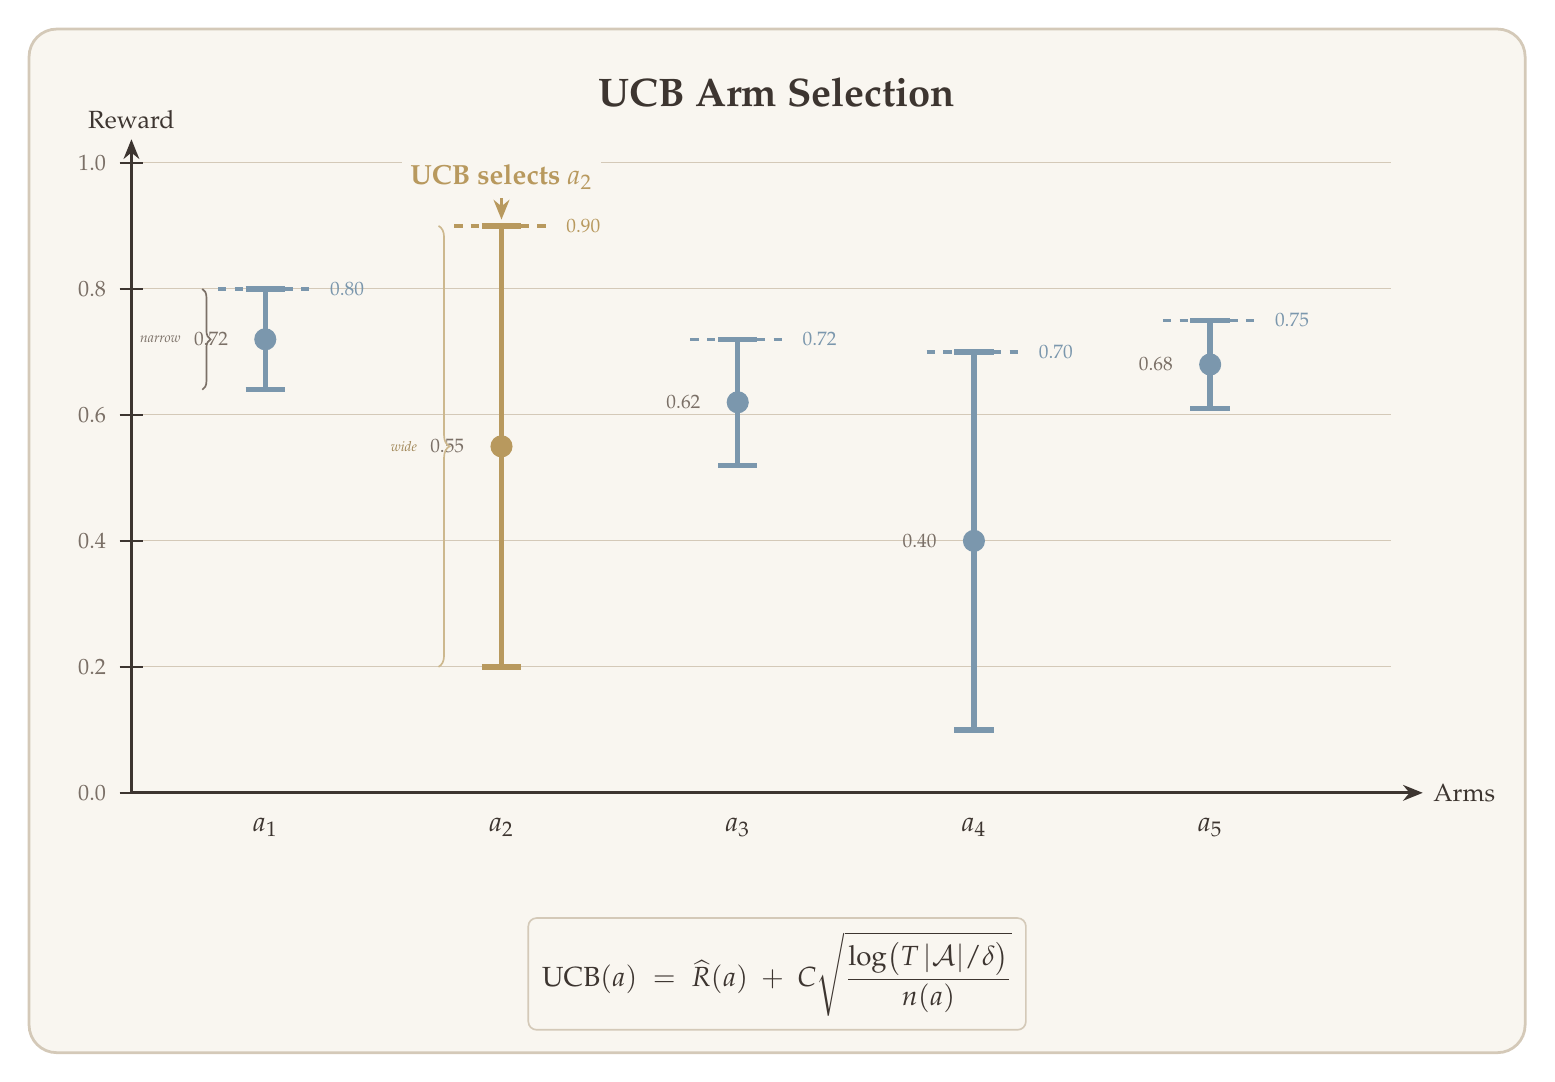
\begin{tikzpicture}[
  >={Stealth[length=2.5mm, width=2mm]},
]

% ── Dimensions ──
% Canvas approximately 18cm wide x 11cm tall
% x: 0..18,  y: 0..11
% Reward axis: y maps [0, 1.0] -> [1.5, 9.5]  (8 cm range)
% Arms at x = 2.5, 5.5, 8.5, 11.5, 14.5  (spacing 3cm, bar width ~1.2cm)

% ── Scaling helpers ──
% reward r  ->  y = 1.5 + 8*r
% So r=0 -> y=1.5,  r=0.5 -> y=5.5,  r=1.0 -> y=9.5

% ── Background ──
\fill[cream, rounded corners=10pt] (-0.5,-1.8) rectangle (18.5,11.2);
\draw[border, rounded corners=10pt, line width=1pt] (-0.5,-1.8) rectangle (18.5,11.2);

% ── Title ──
\node[font=\Large\bfseries, text=dkbrown] at (9,10.4)
  {UCB Arm Selection};

% ── Axes ──
\draw[->, line width=1pt, dkbrown] (0.8,1.5) -- (17.2,1.5)
  node[right, font=\small, text=dkbrown] {Arms};
\draw[->, line width=1pt, dkbrown] (0.8,1.5) -- (0.8,9.8)
  node[above, font=\small, text=dkbrown] {Reward};

% Y-axis ticks
\foreach \r/\lab in {0.0/$0.0$, 0.2/$0.2$, 0.4/$0.4$, 0.6/$0.6$, 0.8/$0.8$, 1.0/$1.0$} {
  \pgfmathsetmacro{\yy}{1.5 + 8*\r}
  \draw[dkbrown, line width=0.6pt] (0.65,\yy) -- (0.95,\yy);
  \node[font=\footnotesize, text=wmgray, left] at (0.6,\yy) {\lab};
}

% Light horizontal grid lines
\foreach \r in {0.2, 0.4, 0.6, 0.8, 1.0} {
  \pgfmathsetmacro{\yy}{1.5 + 8*\r}
  \draw[border, line width=0.4pt] (0.95,\yy) -- (16.8,\yy);
}

% ══════════════════════════════════════════════════
% ARM DATA
% Arm   xc    Rhat   b     UCB   color
% a1    2.5   0.72   0.08  0.80  stblue
% a2    5.5   0.55   0.35  0.90  rwgold  (selected)
% a3    8.5   0.62   0.10  0.72  stblue
% a4   11.5   0.40   0.30  0.70  stblue
% a5   14.5   0.68   0.07  0.75  stblue
% ══════════════════════════════════════════════════

% ── Macro for one arm ──
% #1 = x center, #2 = Rhat, #3 = b, #4 = arm label, #5 = color
\newcommand{\drawarm}[5]{%
  \pgfmathsetmacro{\ymean}{1.5 + 8*#2}%
  \pgfmathsetmacro{\ylo}{1.5 + 8*(#2 - #3)}%
  \pgfmathsetmacro{\yhi}{1.5 + 8*(#2 + #3)}%
  % Confidence interval vertical line
  \draw[#5, line width=2pt] (#1,\ylo) -- (#1,\yhi);
  % CI caps
  \draw[#5, line width=2pt] (#1-0.25,\ylo) -- (#1+0.25,\ylo);
  \draw[#5, line width=2pt] (#1-0.25,\yhi) -- (#1+0.25,\yhi);
  % Mean dot
  \fill[#5] (#1,\ymean) circle (4pt);
  % UCB dashed line at top of CI
  \draw[#5, line width=1.2pt, dashed] (#1-0.6,\yhi) -- (#1+0.6,\yhi);
  % Arm label below axis
  \node[font=\normalsize\bfseries, text=dkbrown, below] at (#1,1.3) {$#4$};
}

% ── Draw each arm ──
% a1: Rhat=0.72, b=0.08, stblue
\drawarm{2.5}{0.72}{0.08}{a_1}{stblue}

% a2: Rhat=0.55, b=0.35, rwgold (highlighted)
\drawarm{5.5}{0.55}{0.35}{a_2}{rwgold}

% a3: Rhat=0.62, b=0.10, stblue
\drawarm{8.5}{0.62}{0.10}{a_3}{stblue}

% a4: Rhat=0.40, b=0.30, stblue
\drawarm{11.5}{0.40}{0.30}{a_4}{stblue}

% a5: Rhat=0.68, b=0.07, stblue
\drawarm{14.5}{0.68}{0.07}{a_5}{stblue}

% ── UCB labels next to each dashed line ──
% a1: UCB = 0.80
\pgfmathsetmacro{\yucbA}{1.5 + 8*(0.72+0.08)}
\node[font=\scriptsize, text=stblue, right] at (3.2,\yucbA) {$0.80$};

% a2: UCB = 0.90 (highest)
\pgfmathsetmacro{\yucbB}{1.5 + 8*(0.55+0.35)}
\node[font=\scriptsize\bfseries, text=rwgold, right] at (6.2,\yucbB) {$0.90$};

% a3: UCB = 0.72
\pgfmathsetmacro{\yucbC}{1.5 + 8*(0.62+0.10)}
\node[font=\scriptsize, text=stblue, right] at (9.2,\yucbC) {$0.72$};

% a4: UCB = 0.70
\pgfmathsetmacro{\yucbD}{1.5 + 8*(0.40+0.30)}
\node[font=\scriptsize, text=stblue, right] at (12.2,\yucbD) {$0.70$};

% a5: UCB = 0.75
\pgfmathsetmacro{\yucbE}{1.5 + 8*(0.68+0.07)}
\node[font=\scriptsize, text=stblue, right] at (15.2,\yucbE) {$0.75$};

% ── Annotation: mean labels (Rhat values) ──
\pgfmathsetmacro{\ymA}{1.5 + 8*0.72}
\node[font=\scriptsize, text=wmgray, left] at (2.15,\ymA) {$0.72$};

\pgfmathsetmacro{\ymB}{1.5 + 8*0.55}
\node[font=\scriptsize, text=wmgray, left] at (5.15,\ymB) {$0.55$};

\pgfmathsetmacro{\ymC}{1.5 + 8*0.62}
\node[font=\scriptsize, text=wmgray, left] at (8.15,\ymC) {$0.62$};

\pgfmathsetmacro{\ymD}{1.5 + 8*0.40}
\node[font=\scriptsize, text=wmgray, left] at (11.15,\ymD) {$0.40$};

\pgfmathsetmacro{\ymE}{1.5 + 8*0.68}
\node[font=\scriptsize, text=wmgray, left] at (14.15,\ymE) {$0.68$};

% ── "UCB selects a2" callout ──
\pgfmathsetmacro{\yselect}{1.5 + 8*0.90}
\node[font=\normalsize\bfseries, text=rwgold,
      fill=cream, inner sep=3pt, rounded corners=2pt,
      above] at (5.5,\yselect+0.35) {UCB selects $a_2$};
\draw[->, rwgold, line width=1.2pt] (5.5,\yselect+0.35) -- (5.5,\yselect+0.08);

% ── Brace annotations for "well explored" vs "poorly explored" ──
% a1: well explored (narrow CI)
\pgfmathsetmacro{\yloA}{1.5 + 8*(0.72-0.08)}
\pgfmathsetmacro{\yhiA}{1.5 + 8*(0.72+0.08)}
\draw[decorate, decoration={brace, amplitude=3pt, mirror}, wmgray, line width=0.6pt]
  (1.7,\yloA) -- (1.7,\yhiA);
\node[font=\tiny\itshape, text=wmgray, left, align=right] at (1.55,\ymA) {narrow};

% a2: poorly explored (wide CI)
\pgfmathsetmacro{\yloB}{1.5 + 8*(0.55-0.35)}
\pgfmathsetmacro{\yhiB}{1.5 + 8*(0.55+0.35)}
\draw[decorate, decoration={brace, amplitude=4pt, mirror}, rwgold!70, line width=0.6pt]
  (4.7,\yloB) -- (4.7,\yhiB);
\node[font=\tiny\itshape, text=rwgold!80!dkbrown, left, align=right] at (4.55,\ymB) {wide};

% ── Formula at the bottom ──
\node[font=\normalsize, text=dkbrown, fill=cream, inner sep=5pt, rounded corners=3pt,
      draw=border, line width=0.6pt] at (9,-0.8)
  {$\displaystyle \mathrm{UCB}(a) \;=\; \widehat{R}(a) \;+\;
    C\sqrt{\frac{\log\bigl(T\,|\mathcal{A}|/\delta\bigr)}{n(a)}}$};

\end{tikzpicture}
\end{document}
